% !TEX encoding = UTF-8 Unicode
% !TEX root = ../Saunkin.tex

\chapter{Evaluation} \label{c4:evaluation}

This chapter evaluates the results produced by the system: given an author, return the counts of their total citations by contribution category.
Each author represents an atomic use case, where the entirety of their publications is considered at the time of evaluation.
Section~\ref{sec:classification-checks} evaluates the classification algorithm in isolation, by comparing the output of the respective function to manually counted citations for a single use case.
Section~\ref{sec:data-source-comparison} compares the data and results of the same author, retrieved from different providers.

\section{Citation classification} \label{sec:classification-checks}

To evaluate the work of the citation classification function, let us consider an author, for instance \emph{Spiros Skiadopoulos}.
Following the implemented methodology, described in Section~\ref{sec:processing-pipeline}, the evaluation is carried out in the context of a single provider, for instance \emph{OpenAlex}.

The classification function compares the authors of each cited and citing publication, to calculate the citation classification as \emph{direct}, \emph{co-author} or \emph{external}.

To operate on realistic data, we have retrieved all records from the selected provider for the selected author on 9 October 2026, and stored a normalized citation graph in the local database.
Going forward, to analyze data, we will be using SQL queries and their results; this will help make the evaluation framework clear to understand and reproducible.

Tables~\ref{tab:sample-publications}--\ref{tab:sample-citations} demonstrate a sample of records in the tables of the local database.


\begin{table}[tb]
    \centering
    \begin{tabular}{|l|l|}
        \hline
        Field & Value \\
        \hline\hline
        provider & openalex \\
        pub\_id & W3141363959 \\
        title & inTIME: A Machine Learning-Based Framework for \dots \\
        normalised\_title & intime: a machine learning-based framework for \dots \\
        external\_id & https://doi.org/10.3390/electronics10070818 \\
        year & 2021 \\
        citation\_count & \\
        \hline
    \end{tabular}
    \caption{A sample record of the \texttt{publications} table}
    \label{tab:sample-publications}
\end{table}

\begin{table}[tb]
    \centering
    \footnotesize
    \begin{tabular}{|l|l|l|l|l|}
        \hline
        provider & author\_id & original\_name & normalised\_name & organisation \\
        \hline\hline
        openalex & A5046481193 & Paris Koloveas & paris koloveas & University of Peloponnese \\
        openalex & A5054180455 & Thanasis Chantzios & thanasis chantzios & University of Peloponnese \\
        \hline
    \end{tabular}
    \caption{Sample records of the \texttt{authors} table}
    \label{tab:sample-authors}
\end{table}

\begin{table}[tb]
    \centering
    \begin{tabular}{|l|l|l|r|}
        \hline
        provider & pub\_id & author\_id & position \\
        \hline\hline
        openalex & W3141363959 & A5046481193 & 1 \\
        openalex & W3141363959 & A5054180455 & 2 \\
        \hline
    \end{tabular}
    \caption{Sample records of the \texttt{contributions} table}
    \label{tab:sample-contributions}
\end{table}

\begin{table}[tb]
    \centering
    \begin{tabular}{|l|l|l|}
        \hline
        provider & source\_pub\_id & target\_pub\_id \\
        \hline\hline
        openalex & W4386028955 & W3141363959 \\
        openalex & W4200158199 & W3141363959 \\
        \hline
    \end{tabular}
    \caption{Sample records of the \texttt{citations} table}
    \label{tab:sample-citations}
\end{table}

Each of the steps below defines a named query, building on the previously defined named queries.
The complete query is built at the end, combining all the steps and producing the final result.

The selected author is found in the \texttt{authors} table.

\begin{quote}
    \begin{vercode}
WITH selected_author AS (
    SELECT *
    FROM authors
    WHERE provider = 'openalex'
        AND normalised_name = 'spiros skiadopoulos'
)
    \end{vercode}
\end{quote}

\begin{center}
    \begin{tabular}{|l|l|}
        \hline
        Column & Value \\
        \hline\hline
        provider & openalex \\
        author\_id & A5009411092 \\
        original\_name & Spiros Skiadopoulos \\
        normalised\_name & spiros skiadopoulos \\
        organisation & University of Peloponnese \\
        \hline
    \end{tabular}
\end{center}

The selected author has multiple records in the \texttt{contributions} table.

\begin{quote}
    \begin{vercode}
WITH author_contributions AS (
    SELECT c.*
    FROM contributions c
        JOIN selected_author sa
            ON c.provider = sa.provider
                AND c.author_id = sa.author_id
)
    \end{vercode}
\end{quote}

\begin{center}
    \begin{tabular}{|l|l|l|r|}
        \hline
        provider & pub\_id & author\_id & position \\
        \hline\hline
        openalex & W129833210 & A5009411092 & 3 \\
        openalex & W141810174 & A5009411092 & 3 \\
        \multicolumn{4}{|c|}{$\vdots$} \\
        \multicolumn{4}{|c|}{Total: 117 records} \\
        \hline
    \end{tabular}
\end{center}

The selected author's publication citations are stored in the \texttt{citations} table.
The column \texttt{target\_pub\_id} indicates that these are all incoming citations.

\begin{quote}
    \begin{vercode}
WITH author_citations AS (
    SELECT ci.*
    FROM citations ci
        JOIN author_contributions ac
            ON ci.provider = ac.provider
                AND ci.target_pub_id = ac.pub_id
)
    \end{vercode}
\end{quote}

\begin{center}
    \begin{tabular}{|r|}
        \hline
        num\_citations\_total \\
        \hline\hline
        3584 \\
        \hline
    \end{tabular}
\end{center}

We select \emph{direct} citations from all author citations by matching the author contributions with the \texttt{source\_pub\_id} of the author citations.

\begin{quote}
    \begin{vercode}
WITH direct_citations AS (
    SELECT aci.*
    FROM author_citations aci
        JOIN author_contributions ac
            ON aci.provider = ac.provider
                AND aci.source_pub_id = ac.pub_id
)
    \end{vercode}
\end{quote}

\begin{center}
    \begin{tabular}{|r|}
        \hline
        num\_citations\_direct \\
        \hline\hline
        115 \\
        \hline
    \end{tabular}
\end{center}

The remaining citations, where the selected author is not an author of a citing publication, are either \emph{co-author} or \emph{external} citations.

\begin{quote}
    \begin{vercode}
WITH indirect_citations AS (
    SELECT aci.*
    FROM author_citations aci
        LEFT OUTER JOIN direct_citations dc
            ON aci.provider = dc.provider
                AND aci.source_pub_id = dc.source_pub_id
                AND aci.target_pub_id = dc.target_pub_id
    WHERE dc.source_pub_id IS NULL
)
    \end{vercode}
\end{quote}

\begin{center}
    \begin{tabular}{|r|}
        \hline
        num\_citations\_indirect \\
        \hline\hline
        3469 \\
        \hline
    \end{tabular}
\end{center}

The \emph{co-author} citations are those where the citing and cited publications share at least one other author, besides the selected author.

\begin{quote}
    \begin{vercode}
WITH coauthor_citations AS (
    SELECT DISTINCT ic.*
    FROM indirect_citations ic
        JOIN contributions cited
            ON cited.provider = ic.provider
                AND cited.pub_id = ic.target_pub_id
        JOIN contributions citing
            ON citing.provider = ic.provider
                AND citing.pub_id = ic.source_pub_id
                AND citing.author_id = cited.author_id
)
    \end{vercode}
\end{quote}

\begin{center}
    \begin{tabular}{|r|}
        \hline
        num\_citations\_coauthor \\
        \hline\hline
        243 \\
        \hline
    \end{tabular}
\end{center}

The \emph{external} citations are those where the citing and cited publications share no author at all.

\begin{quote}
    \begin{vercode}
WITH external_citations AS (
    SELECT ic.*
    FROM indirect_citations ic
        LEFT OUTER JOIN coauthor_citations cc
            ON ic.provider = cc.provider
                AND ic.source_pub_id = cc.source_pub_id
                AND ic.target_pub_id = cc.target_pub_id
    WHERE cc.source_pub_id IS NULL
)
    \end{vercode}
\end{quote}

\begin{center}
    \begin{tabular}{|r|}
        \hline
        num\_citations\_external \\
        \hline\hline
        3226 \\
        \hline
    \end{tabular}
\end{center}

The complete query combines all the steps above and returns all the counts at once.

\begin{quote}
    \begin{vercode}
WITH
selected_author AS (
    SELECT *
    FROM authors
    WHERE provider = 'openalex'
        AND normalised_name = 'spiros skiadopoulos'
),
author_contributions AS (
    SELECT c.*
    FROM contributions c
        JOIN selected_author sa
            ON c.provider = sa.provider
                AND c.author_id = sa.author_id
),
author_citations AS (
    SELECT ci.*
    FROM citations ci
        JOIN author_contributions ac
            ON ci.provider = ac.provider
                AND ci.target_pub_id = ac.pub_id
),
direct_citations AS (
    SELECT aci.*
    FROM author_citations aci
        JOIN author_contributions ac
            ON aci.provider = ac.provider
                AND aci.source_pub_id = ac.pub_id
),
indirect_citations AS (
    SELECT aci.*
    FROM author_citations aci
        LEFT OUTER JOIN direct_citations dc
            ON aci.provider = dc.provider
                AND aci.source_pub_id = dc.source_pub_id
                AND aci.target_pub_id = dc.target_pub_id
    WHERE dc.source_pub_id IS NULL
),
coauthor_citations AS (
    SELECT DISTINCT ic.*
    FROM indirect_citations ic
        JOIN contributions cited
            ON cited.provider = ic.provider
                AND cited.pub_id = ic.target_pub_id
        JOIN contributions citing
            ON citing.provider = ic.provider
                AND citing.pub_id = ic.source_pub_id
                AND citing.author_id = cited.author_id
),
external_citations AS (
    SELECT ic.*
    FROM indirect_citations ic
        LEFT OUTER JOIN coauthor_citations cc
            ON ic.provider = cc.provider
                AND ic.source_pub_id = cc.source_pub_id
                AND ic.target_pub_id = cc.target_pub_id
    WHERE cc.source_pub_id IS NULL
)
SELECT
    (SELECT COUNT(*) FROM author_citations)
        AS num_citations_total,
    (SELECT COUNT(*) FROM direct_citations)
        AS num_citations_direct,
    (SELECT COUNT(*) FROM coauthor_citations)
        AS num_citations_coauthor,
    (SELECT COUNT(*) FROM external_citations)
        AS num_citations_external;
    \end{vercode}
\end{quote}

\begin{center}
    \begin{tabular}{|r|r|r|r|}
        \hline
        total & direct & co-author & external \\
        \hline\hline
        3584 & 115 & 243 & 3226 \\
        \hline
    \end{tabular}
\end{center}

Figure~\ref{fig:sample-counts} shows the counts calculated by the system for the same author and provider.
The three subtotals produce the expected total ($115 + 243 + 3226 = 3584$), matching the system counts.

\begin{figure}[tb]
    \centering
    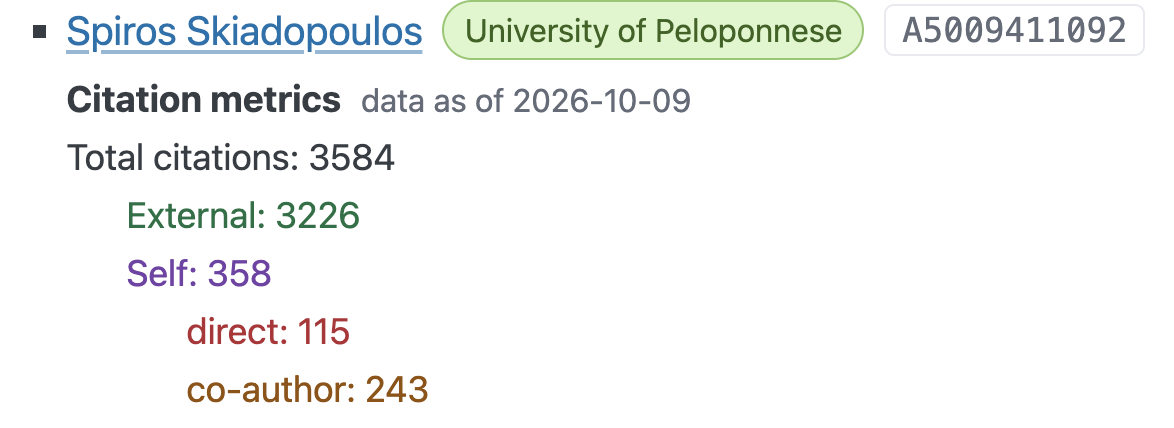
\includegraphics[scale=.4]{include/fig-sample-counts}
    \caption{Sample counts calculated by the system}
    \label{fig:sample-counts}
\end{figure}

\section{Comparison of data sources} \label{sec:data-source-comparison}

To evaluate and compare the data sources, we used a sample of one author and searched the same author with each of the providers.
The identifiers below represent the same author, \emph{Spiros Skiadopoulos}, as returned from different providers: \texttt{A5009411092} from \textsf{OpenAlex}, \texttt{1688897} from \textsf{Semantic Scholar} and \texttt{fxBHpbgAAAAJ} from \textsf{Google Scholar}.
All data were updated on the same date, 10 October 2026.

None of the provider data or the produced counts match precisely.

Table~\ref{tab:provider-distribution} illustrates the distribution of the publications of the selected author across the providers.
As each provider exposes their own publication identifier, and in an attempt to compare the papers returned by each source, we compared publications by normalized title, and discovered that there are 236 distinct titles for the same author in total, where only 71 match across all providers.

\begin{table}[tb]
    \centering
    \begin{minipage}[c]{0.6\linewidth}
        \centering
        \small
        \begin{tabular}{|l|r|}
            \hline
            Publications (by normalized\_title) & Count \\
            \hline\hline
            on any provider (union) & 236 \\
            on all providers (intersection) & 71 \\
            exclusive to \textsf{OpenAlex} & 12 \\
            exclusive to \textsf{Semantic Scholar} & 101 \\
            exclusive to \textsf{Google Scholar} & 32 \\
            \hline
        \end{tabular}
    \end{minipage}

    \medskip
    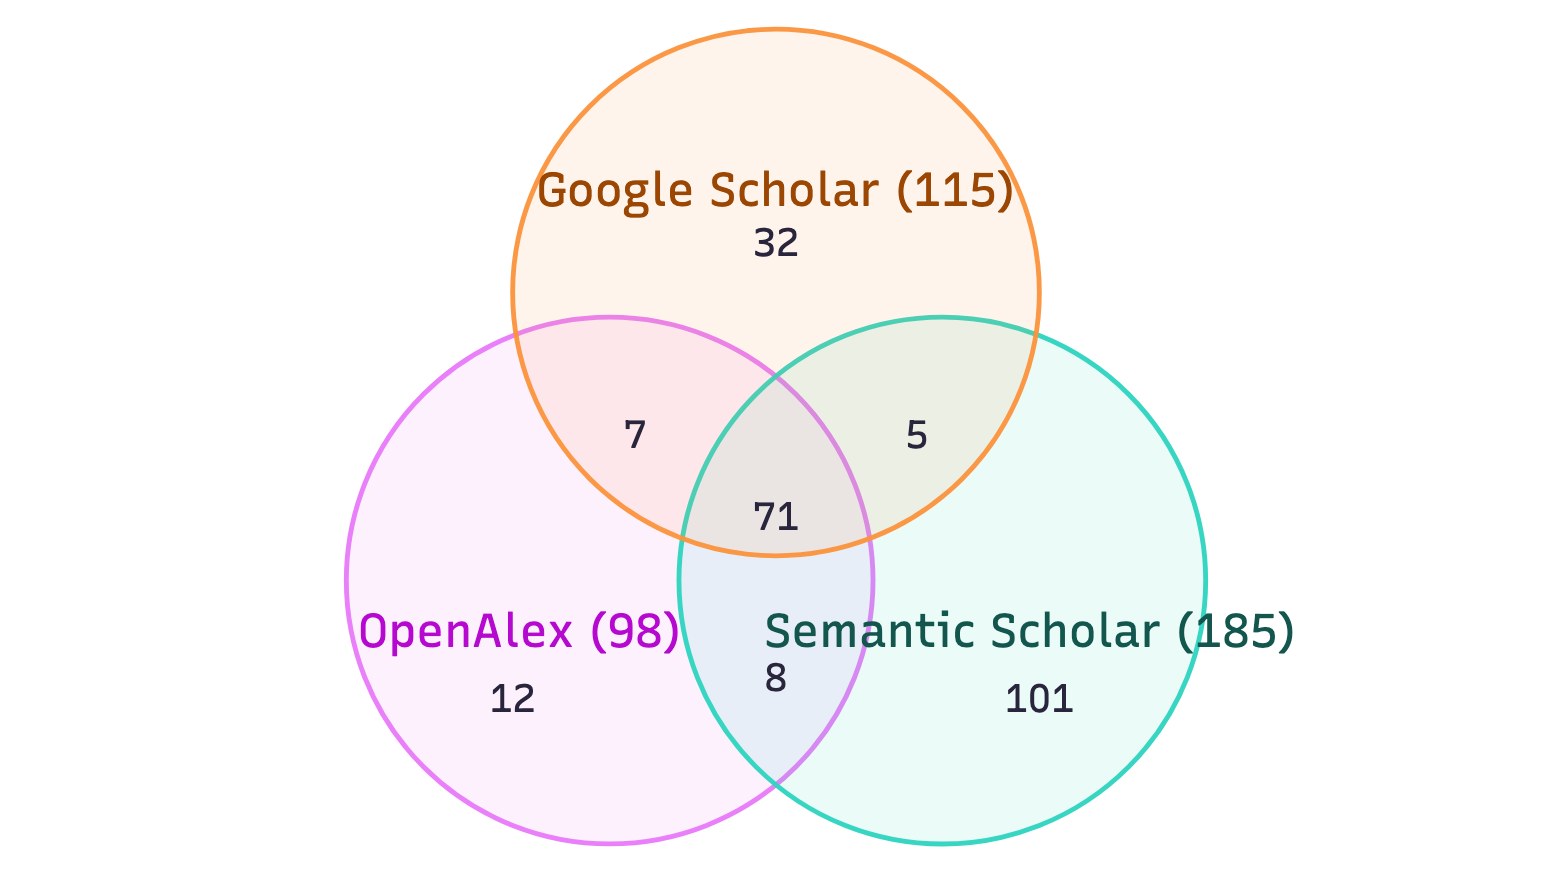
\includegraphics[scale=.2]{include/fig-provider-distribution-diagram}
    \caption{Distribution of author publications by source}
    \label{tab:provider-distribution}
\end{table}

Table~\ref{tab:provider-comparison} contains the publication and citation counts, per provider.

\begin{table}[tb]
    \centering
    \footnotesize
    \setlength{\tabcolsep}{3pt}
    \begin{tabular}{|l|r|r|r|r|r|r|r|r|}
        \hline
        Provider & \shortstack{Publi-\\cations} & \shortstack{With\\citations} & \shortstack{Without\\citations} & Citations & \shortstack{Self-\\citations} & Direct & Co-author & External \\
        \hline\hline
        \textsf{OpenAlex} & 117 & 85 & 32 & 3584 & \shortstack[r]{358\\(10.0\%)} & \shortstack[r]{115\\(3.2\%)} & \shortstack[r]{243\\(6.8\%)} & \shortstack[r]{3226\\(90.0\%)} \\
        \textsf{Semantic Scholar} & 187 & 104 & 83 & 4093 & \shortstack[r]{351\\(8.6\%)} & \shortstack[r]{96\\(2.3\%)} & \shortstack[r]{255\\(6.2\%)} & \shortstack[r]{3742\\(91.4\%)} \\
        \textsf{Google Scholar} & 157 & 86 & 71 & 5458 & \shortstack[r]{76\\(1.4\%)} & \shortstack[r]{76\\(1.4\%)} & \shortstack[r]{0\\(0.0\%)} & \shortstack[r]{5382\\(98.6\%)} \\
        \hline
    \end{tabular}
    \caption{Publication and citation counts for \emph{Spiros Skiadopoulos}, by provider}
    \label{tab:provider-comparison}
\end{table}

All three providers include papers for which no citations were found: 32/117 in \textsf{OpenAlex}, 83/187 in \textsf{Semantic Scholar} and 71/157 in \textsf{Google Scholar} (mainly these are duplicates and alternative versions of cited papers)..
The most cited papers of the selected author are \emph{Conceptual modeling for ETL processes} and \emph{PRIVE: anonymous location-based queries in distributed mobile systems}, across all sources.

In broad terms, the \textsf{OpenAlex} and \textsf{Semantic Scholar} numbers are the closest.
\textsf{Semantic Scholar} returned more papers and more citations than \textsf{OpenAlex} in absolute numbers, but the proportions are similar, as shown in Table~\ref{tab:provider-comparison}.
At the same time, \textsf{Google Scholar} returned more citations than the other two, though very few were classified as self-citations ($<$\,2\%), and all of them as \textsf{direct}.

\textsf{OpenAlex} and \textsf{Semantic Scholar} produced the same classification for 1798/1811 (99\%) citations, including all 57 \textsf{direct}.
The remaining 13 citations alternate between \textsf{co-author} and \textsf{external}, depending on the way providers resolve citing authors.

\textsf{Google Scholar} numbers stand out and seem misleading, compared to either of the other two providers, where author identities are available.

\begin{description}
    \item [Compared to \textsf{OpenAlex}] all citations classified as \textsf{co-author}, and almost half (29/65) of those classified as \textsf{direct}, are \textsf{external} in \textsf{Google Scholar}.
    \item [Compared to \textsf{Semantic Scholar}] almost all (165/167) \textsf{co-author} citations, and almost half (25/57) \textsf{direct} ones, are \textsf{external} in \textsf{Google Scholar}.
\end{description}

For \textsf{Google Scholar} the classification relies on matching authors by plain text names, as described in Section~\ref{sec:data}.
This results in citations classified as \textsf{direct} when the author under analysis is on the citing publication; otherwise the citation is classified as \textsf{external}.
The citing papers do not always include the profile identifier, resulting in even fewer matches for \textsf{direct}.

The following examples demonstrate the differences.

The first example is the citation discussed in Chapter~\ref{c1:intro}, where publication~\cite{Kalnis2007} cites publication~\cite{Ghinita2007}.
\textsf{OpenAlex} and \textsf{Semantic Scholar} return author identities for both papers, so for Spiros Skiadopoulos the citation is classified as \textsf{co-author}.
For \textsf{Google Scholar} data, the same citation is classified as \textsf{external}.
Listing~\ref{lst:example-coauthor} shows the parsed data from the responses.

\begin{lstlisting}[float=tb, basicstyle=\footnotesize\ttfamily, caption={Authors of {[GPK2007]} and {[KGMP2007]}, as returned by providers}, label={lst:example-coauthor}]
// OpenAlex - [GPK2007]
[["A5069236544", "Gabriel Ghinita"], ["A5014399734", "Panos Kalnis"],
 ["A5009411092", "Spiros Skiadopoulos"]]
// OpenAlex - [KGMP2007]
[["A5014399734", "Panos Kalnis"], ["A5069236544", "Gabriel Ghinita"],
 ["A5053720072", "Kyriakos Mouratidis"], ["A5091887420", "Dimitris Papadias"]]

// Semantic Scholar - [GPK2007]
[{"authorId": "2182067502", "name": "G. Ghinita"},
 {"authorId": "2000187", "name": "Panos Kalnis"},
 {"authorId": "1688897", "name": "S. Skiadopoulos"}]
// Semantic Scholar - [KGMP2007]
[{"authorId": "2000187", "name": "Panos Kalnis"},
 {"authorId": "2182067502", "name": "G. Ghinita"},
 {"authorId": "1753946", "name": "K. Mouratidis"},
 {"authorId": "1746338", "name": "Dimitris Papadias"}]

// Google Scholar - [GPK2007]
"authors": "G Ghinita, P Kalnis, S Skiadopoulos"
// Google Scholar - [KGMP2007]
[{"name": "P Kalnis", "author_id": "-NdSrrYAAAAJ"},
 {"name": "G Ghinita", "author_id": "t_AzcmUAAAAJ"},
 {"name": "K Mouratidis", "author_id": "vq5oTnEAAAAJ"}]
\end{lstlisting}

The second example demonstrates provider errors resulting in skewed citation counts.
\textsf{OpenAlex} returns the paper~\cite{Terrovitis2004} as citing itself, which counts as a \textsf{direct} citation.
At the same time, \textsf{Google Scholar} returns \texttt{S Skiadopoulost} as an author for the same work, with nothing else matching this name, and the name matching no profile.
Listing~\ref{lst:example-errors} includes both records.

\begin{lstlisting}[float=tb, basicstyle=\footnotesize\ttfamily, caption={Errors in the responses of \textsf{OpenAlex} and \textsf{Google Scholar}}, label={lst:example-errors}]
// OpenAlex
{"id": "https://openalex.org/W4241330289",
 "title": "Modeling and language support for the management of pattern-bases",
 "publication_year": 2004,
 "referenced_works": [..., "https://openalex.org/W4241330289", ...]}

// Google Scholar
{"result_id": "WY_w50sssDEJ",
 "title": "Modeling and Language Support for the Management of",
 "publication_info": {
   "summary": "S Skiadopoulost, E Bertinos - International Conference on ..., 2004",
   "authors": [{"name": "S Skiadopoulost"}, {"name": "E Bertinos"}]}}
\end{lstlisting}

Having analyzed one sample author, we have shown that the data returned by each provider does not overlap precisely with data returned by other providers.
Also, we have demonstrated that none of the sources used in this work was 100\% accurate and curated.
The accuracy of classification counts, derived from inaccurate data, are still a good statisticall approach, though should be treated with care.
